\documentclass[16pt]{article}
\usepackage{graphicx}
\usepackage{amsmath}
\graphicspath{{images/}}



\title{\huge{Analytic Geometry and Calculus I Assignment}}
\author{\huge{Papa Kofi Boahen Roll Number:10211100334}}
\date{\today} 

\begin{document}
	\maketitle
\section*{\underline{Question 1}}
\begin{huge}
	\[ \lim_{x \to 0}f(x) \quad where \quad f(x) = \begin{cases} 
		x + 3, \ & x < 0 \\
		-x + 3, \ & x \geq 0 
	\end{cases}
	\]
\end{huge}	

\begin{figure}[h]
	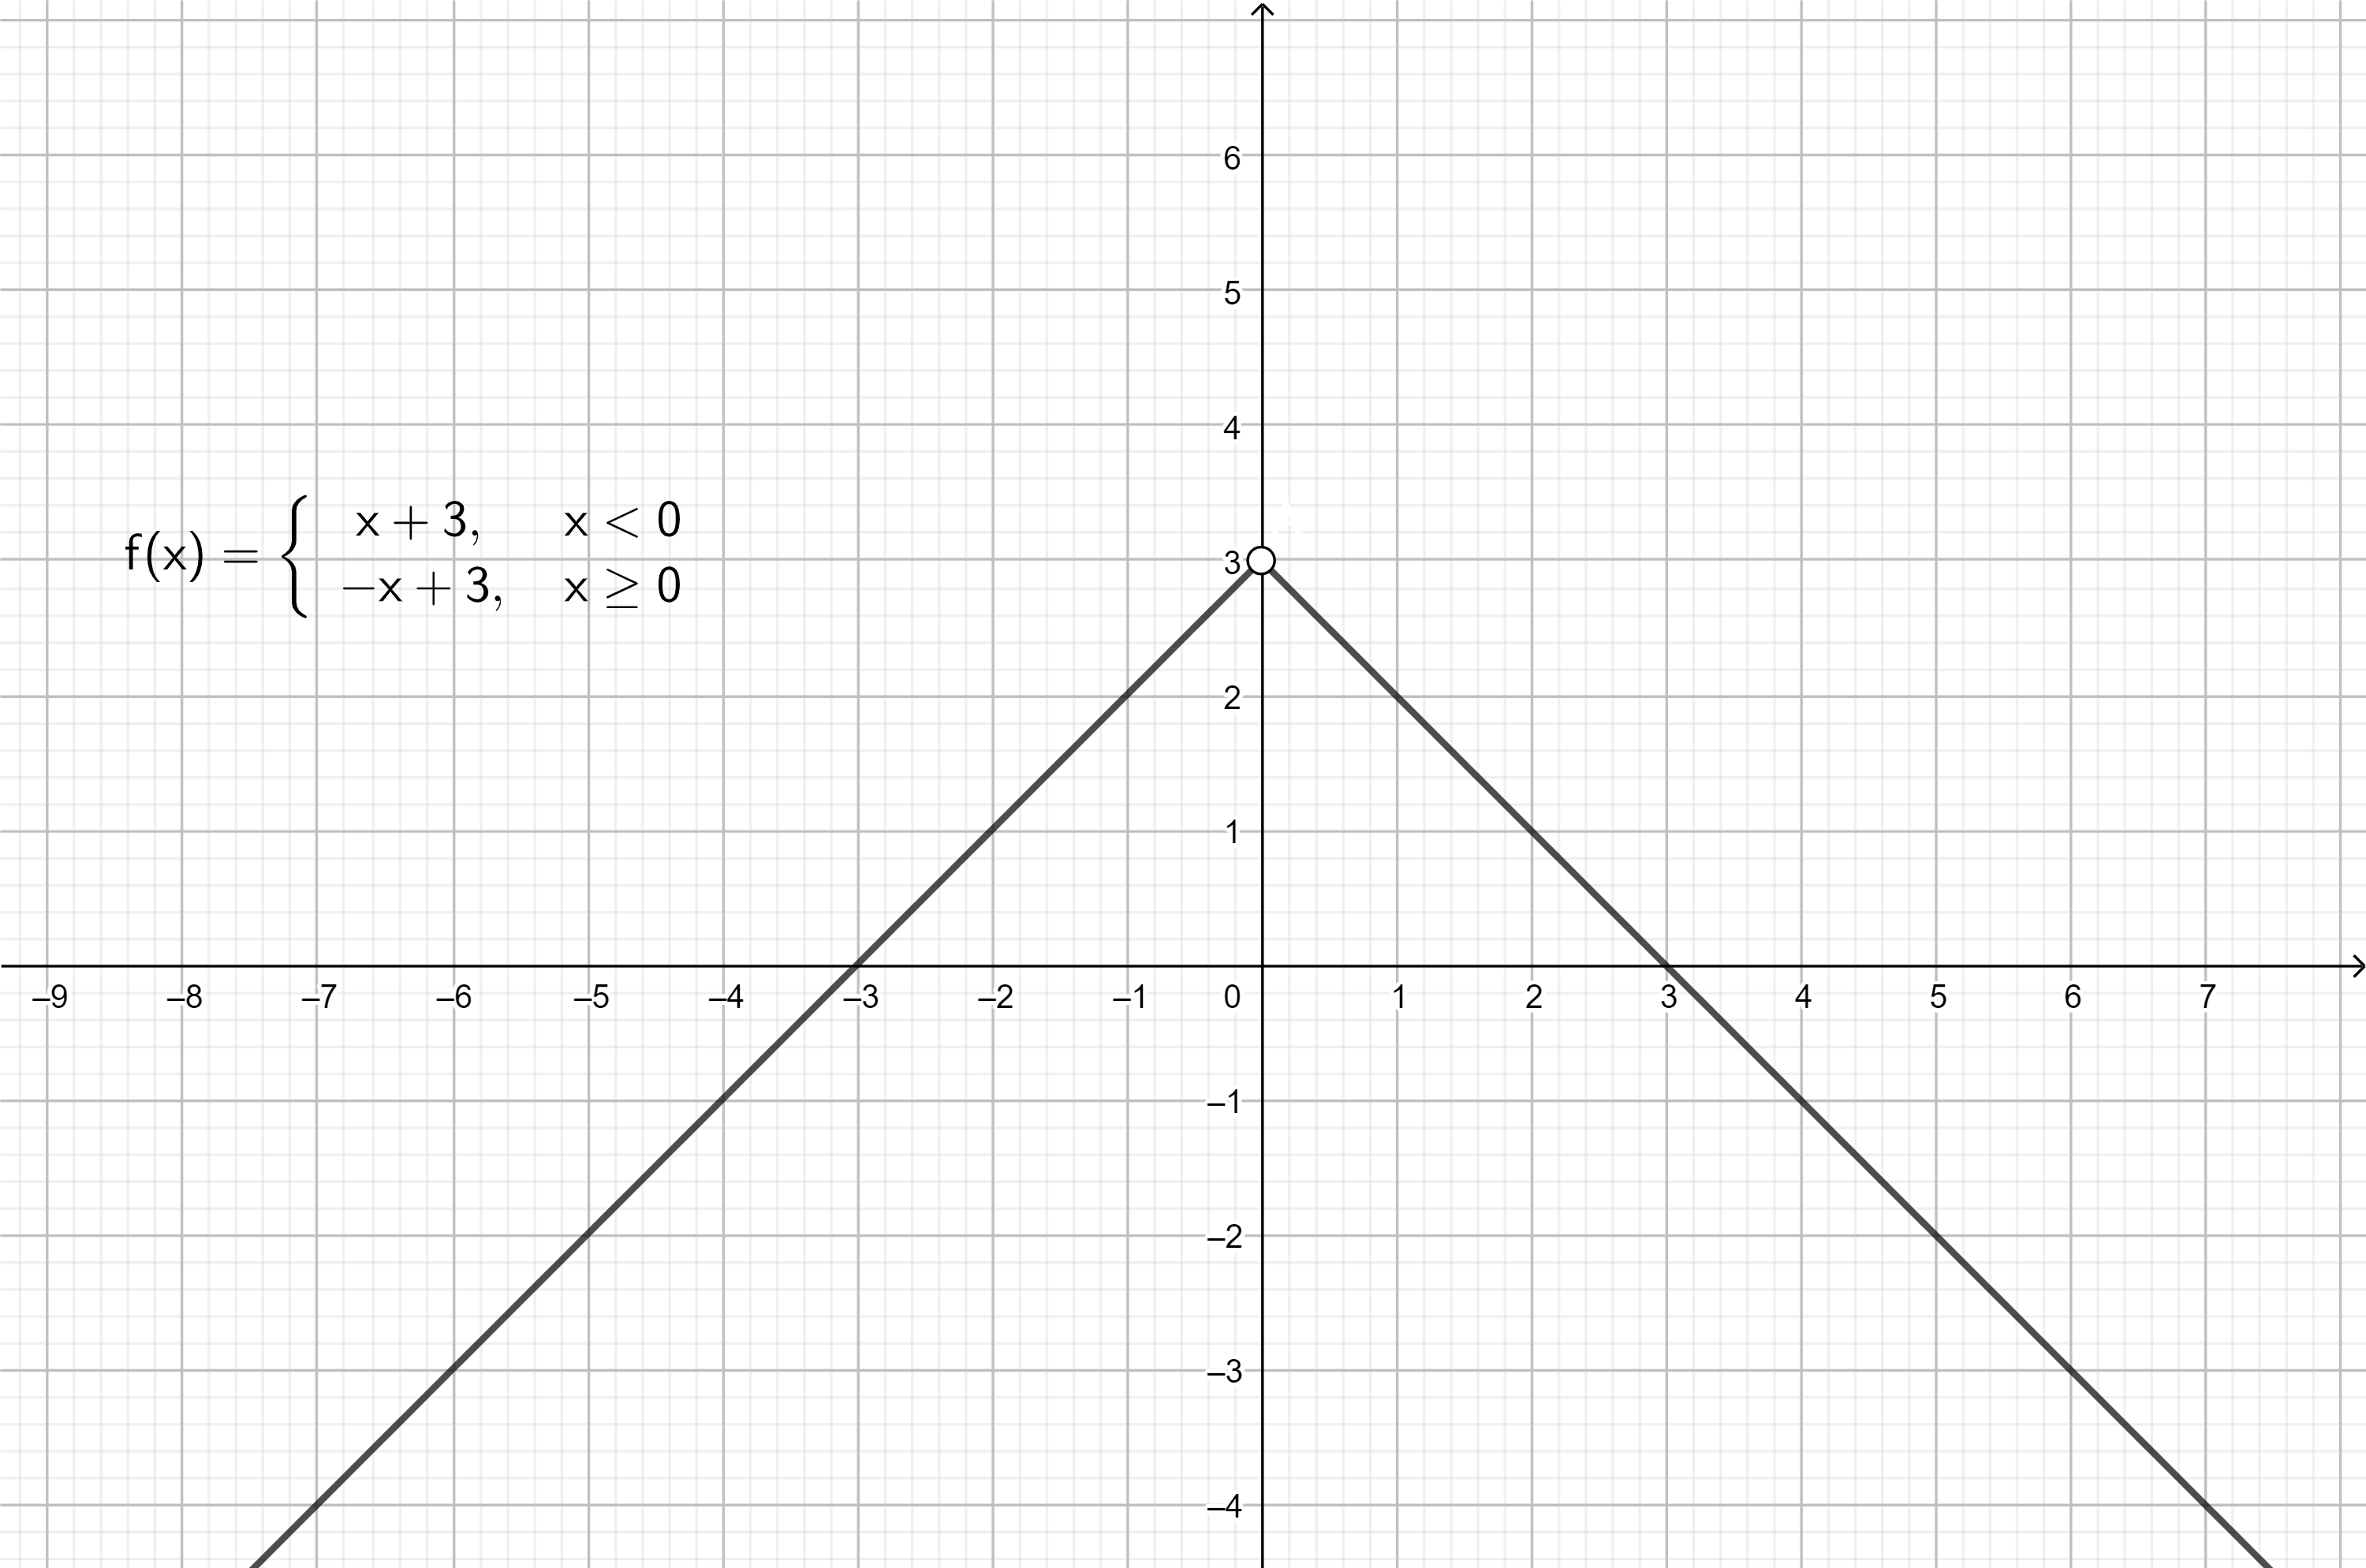
\includegraphics[width=\textwidth]{Graph1.jpg}
	\caption{Graph for Question 1}
	\label{graph1}
\end{figure}

\vspace{1cm}

\huge{Evaluate the one-sided limits.}

\begin{align*}
	\lim_{x\to0^-} f(x) & = \lim_{x\to0^-} (x+3) = 0 + 3 = 3 \\
	&
	\\
	\lim_{x\to0^+} f(x) & =  \lim_{x\to0^+} (-x+3) = -(0) + 3 = 3
\end{align*}
\\
If the one-sided limits are the same then the limit exists. Figure \ref{graph1} confirms this. \\
  \[ \lim_{x \to 0} f(x) = 3 \] \textbf{exists.}

\vspace{2cm}

\section*{\underline{Question 2}}
\begin{huge}
	\[ \lim_{x \to 2}f(x) \quad where \quad f(x) = \begin{cases} 
		x, \ &x < 2 \\
		x + 1, \ &x \geq 2 
	\end{cases}
	\]
\end{huge}

\begin{figure}[h]
	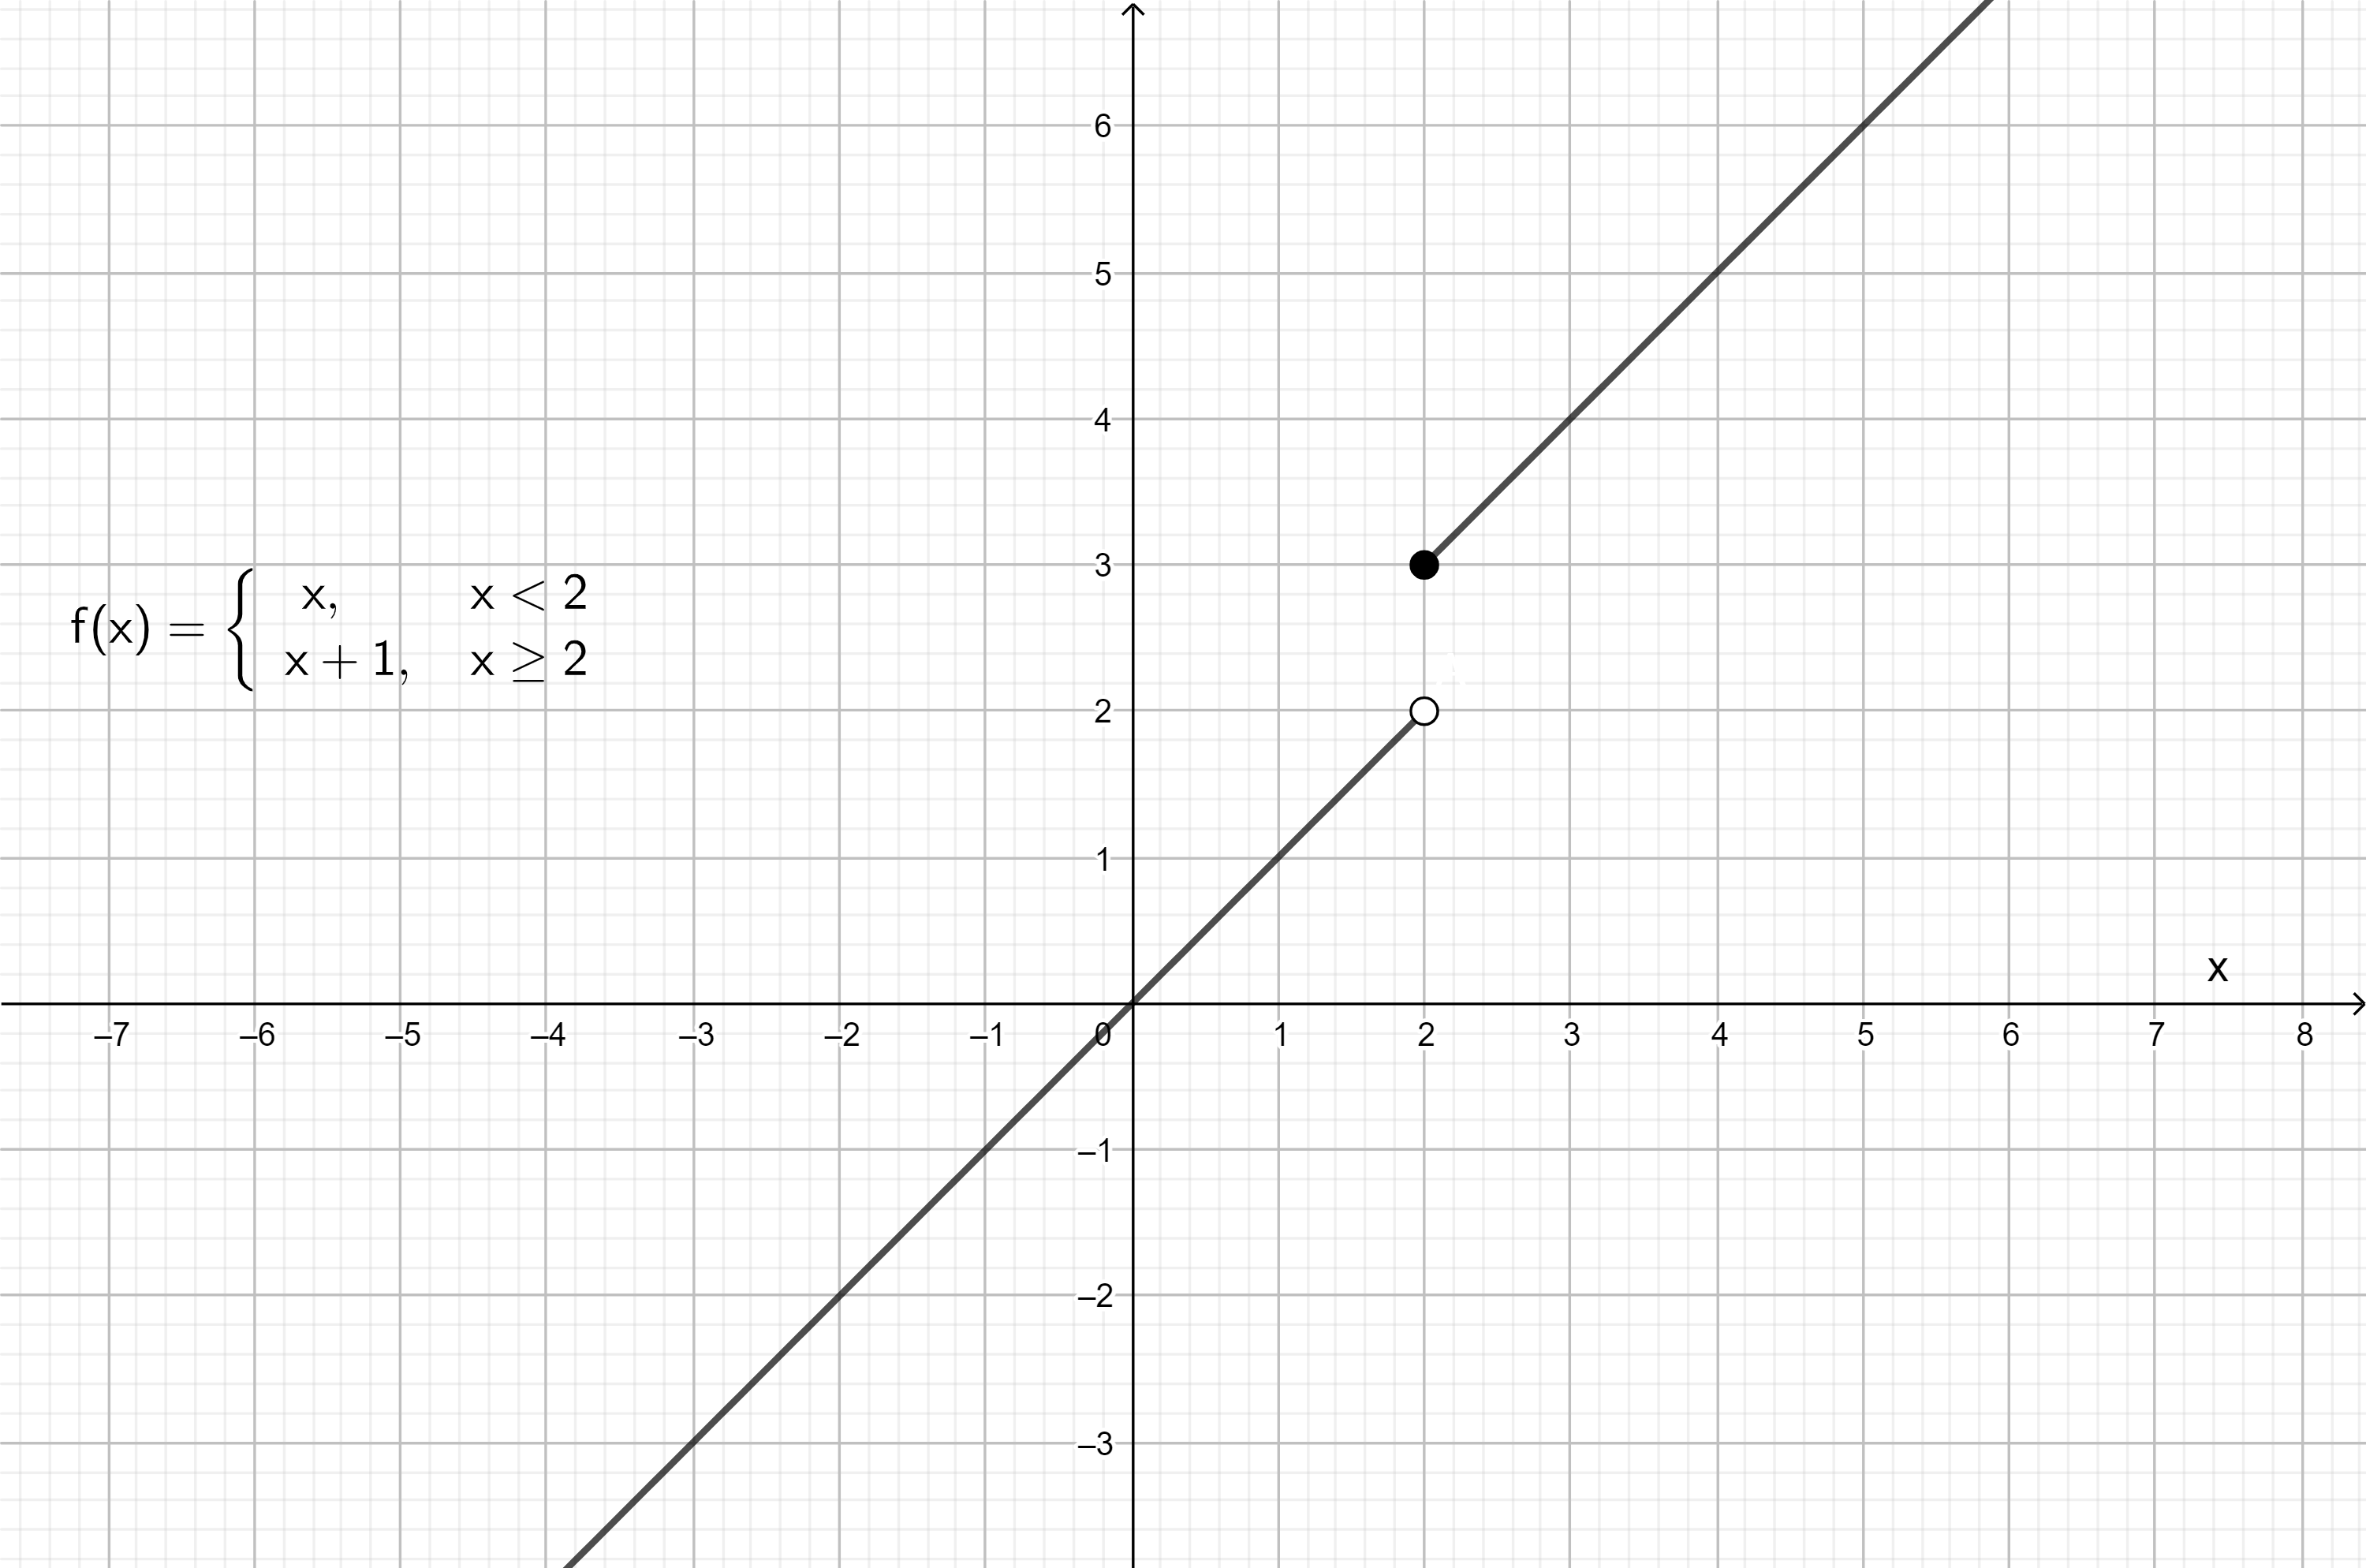
\includegraphics[width=\textwidth]{graph2.jpg}
	\caption{Graph for Question 2}
	\label{graph2}
\end{figure}

\vspace{1cm}

\huge{Evaluate the one-sided limits.}

\begin{align*}
	\lim_{x\to2^-} f(x) & = \lim_{x\to2^-} (x) = 2 = 2 \\
	&
	\\
	\lim_{x\to2^+} f(x) & =  \lim_{x\to2^+} (x+1) = 2 + 1 = 3
\end{align*}
\\
If the one-sided limits are the different then the limit fails to exist. Figure \ref{graph2} confirms this. \\
\[ \displaystyle\lim_{x \to 2} f(x) \] \textbf{does not exist.}

\vspace{2cm}

\section*{\underline{Question 3}}
\begin{huge}
\[ \lim_{x \to 2}f(x) \quad where \quad f(x) = \begin{cases} 
	x^{2} - 2x, \ & x < 2 \\
	1, \ & x = 2 \\
	x^{2} - 6x + 8, \ & x > 2 
\end{cases}
\]
\end{huge}

\begin{figure}[h]
	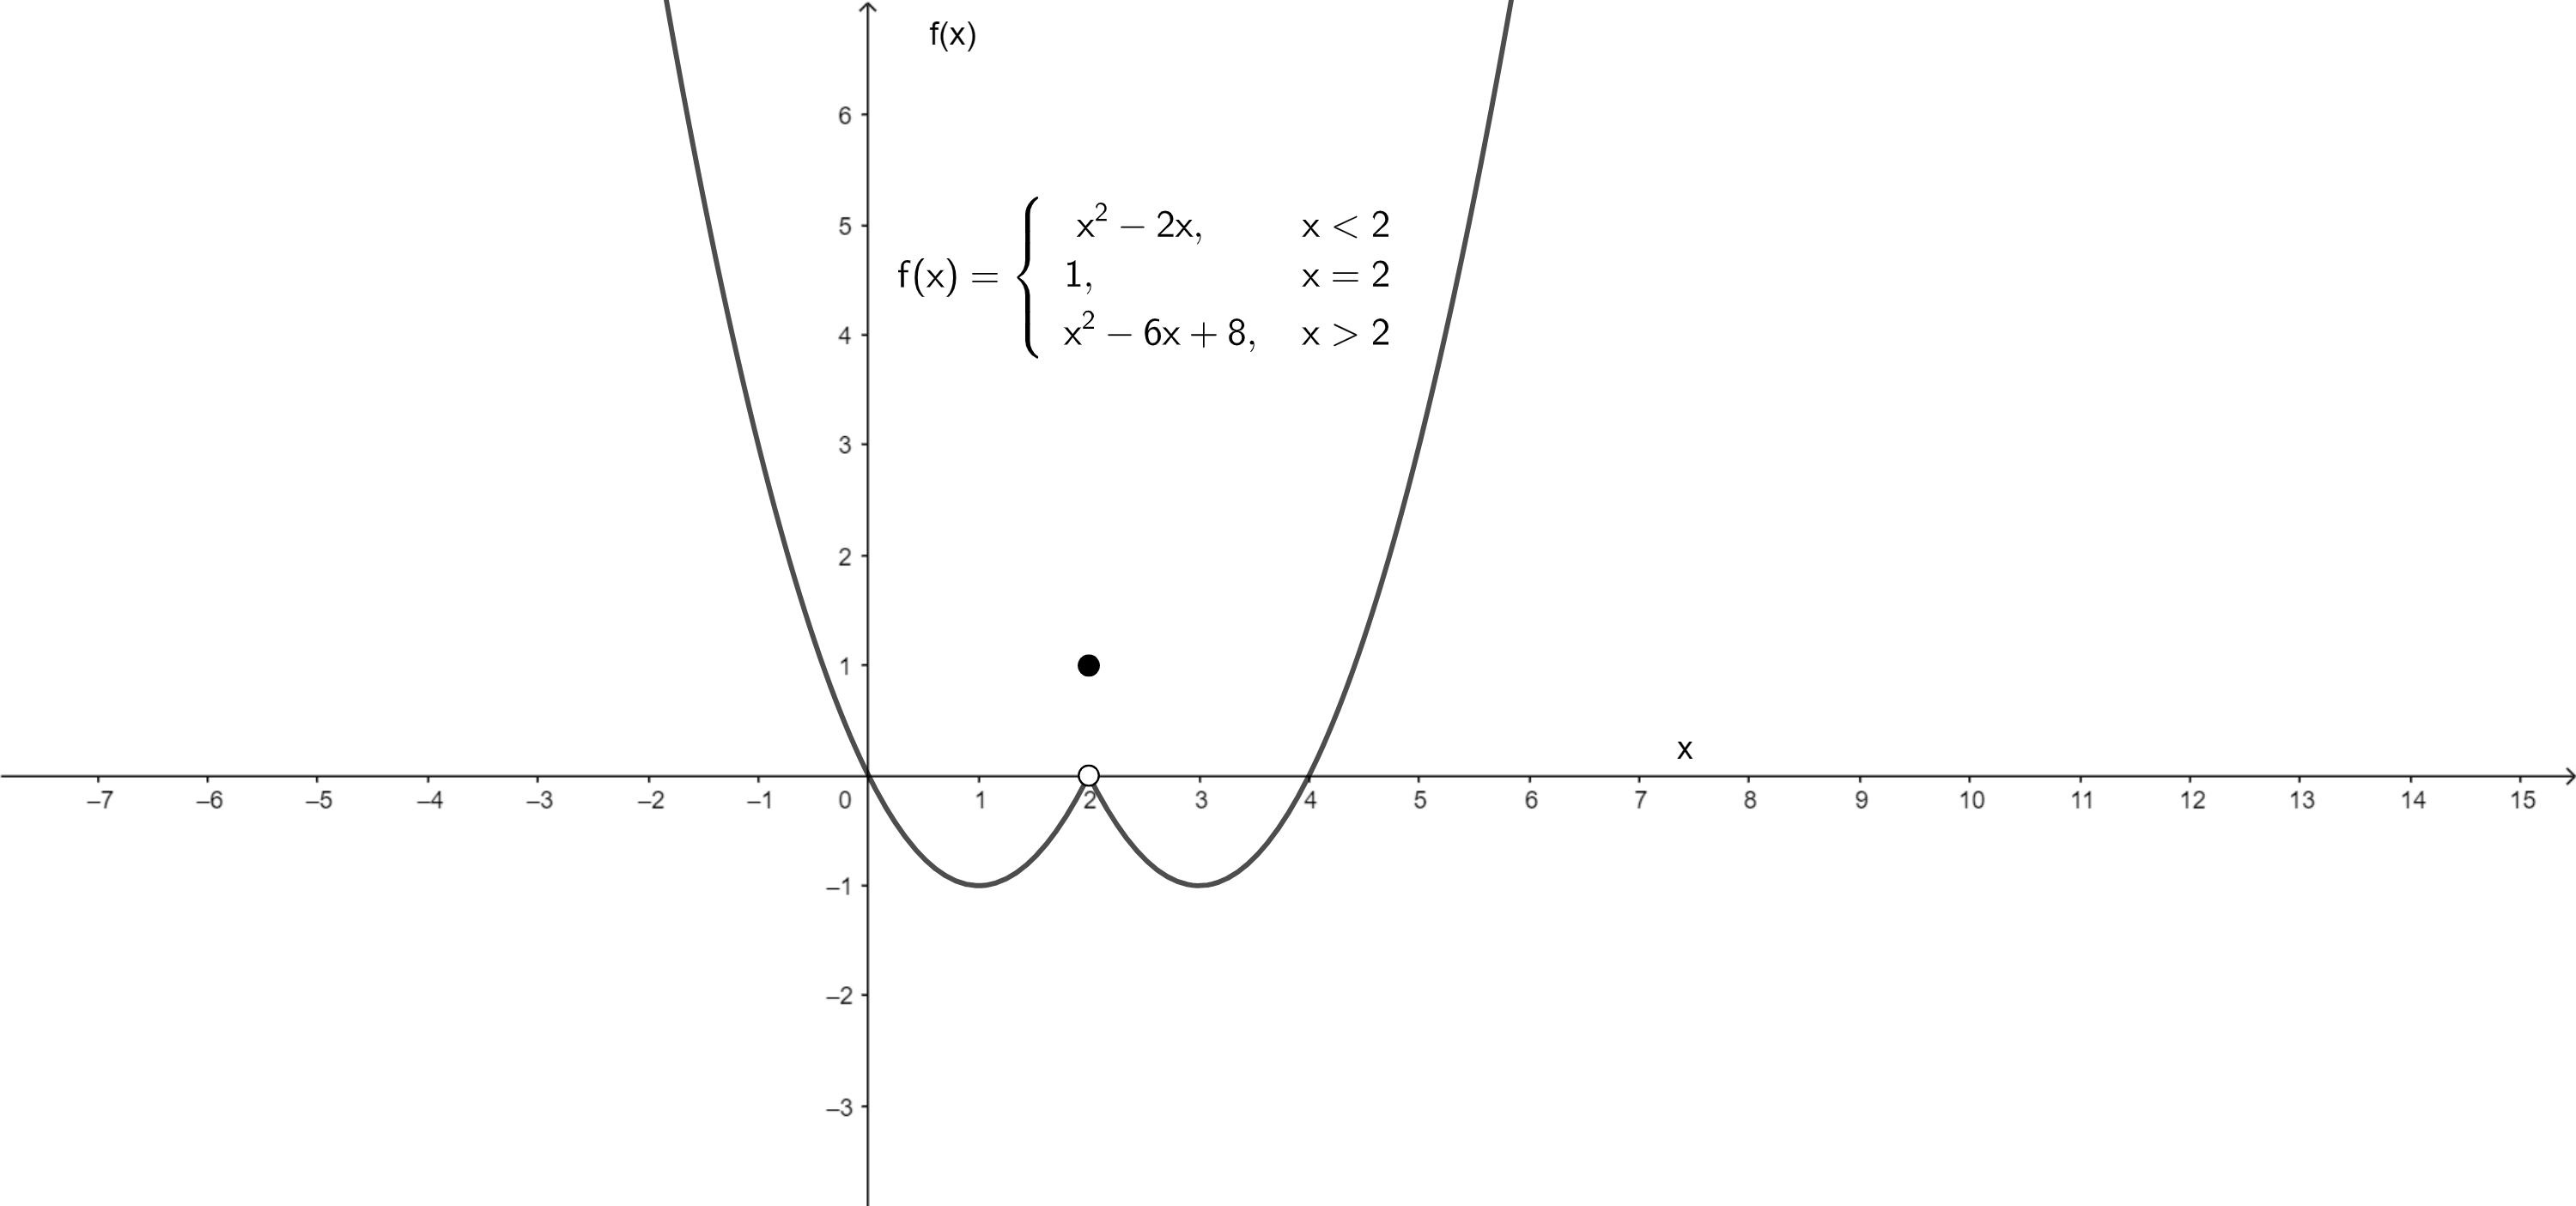
\includegraphics[width=\textwidth]{graph3a.jpg}
	\caption{Graph for Question 3}
	\label{graph3}
\end{figure}

\vspace{1cm}

\huge{Evaluate the one-sided limits.}

\begin{align*}
	\lim_{x\to2^-} f(x) & = \lim_{x\to2^-} (x^2 - 2x) = (2)^2 -2(2) = 0 \\
	&
	\\
	\lim_{x\to2^+} f(x) & =  \lim_{x\to2^+} (x^2 -6x + 8) = (2)^2 -6(2) + 8 = 0
\end{align*}
\\

If the one-sided limits are the same then the limit exists. Figure \ref{graph3} confirms this. \\
\[ \lim_{x \to 2} f(x) = 0 \] \textbf{exists.}


\end{document}